\documentclass[11pt]{article}

\usepackage[T1]{fontenc}
\usepackage[utf8]{inputenc}
\usepackage{mathptmx}
\usepackage[margin=1in]{geometry}
\usepackage{amsmath,amssymb}
\usepackage{graphicx}
\usepackage{booktabs}
\usepackage{tabularx}
\usepackage{multirow}
\usepackage{xcolor}
\usepackage[font=small,labelfont=bf]{caption}
\usepackage{enumitem}
\usepackage{microtype}
\usepackage[section]{placeins}
\usepackage[numbers,sort&compress]{natbib}
\usepackage[colorlinks=true,linkcolor=blue!50!black,citecolor=blue!50!black,urlcolor=blue!50!black]{hyperref}

\graphicspath{{../results/figures/}{../results/analysis/}}
\setlist{itemsep=2pt,topsep=4pt}
\setlength{\parskip}{3pt}

% ---- Links for page 1 ----------------------------------------------------------------------
\newcommand{\repourl}{https://github.com/NJIT-DS677-Deep-Learning/DS677-project}
\newcommand{\demourl}{https://github.com/NJIT-DS677-Deep-Learning/DS677-project/blob/main/demo/demo.ipynb}
\newcommand{\videolink}{\url{https://youtu.be/Y0W7U8WjlfM}}

\newcommand{\file}[1]{\nolinkurl{#1}}
\emergencystretch=1.5em
\newcommand{\vitlite}[1]{ViT-Lite-7/#1}

\title{\textbf{A Small Vision Transformer Trained from Scratch Trails ResNet-18 on CIFAR-10 at Every Patch Size}\\[6pt]
\large A patch-size study with layer analyses}
\author{Rishabh Verma\\[2pt]
\normalsize DS 677 Deep Learning, New Jersey Institute of Technology, Fall 2026\\
\normalsize Model Review and Demo track, Milestone 3 report}
\date{December 2026}

\begin{document}
\maketitle

\begin{center}
\begin{tabular}{@{}rl@{}}
\textbf{Repository:} & \url{\repourl}\\
\textbf{Video presentation:} & \videolink\\
\textbf{Demo notebook:} & \href{\demourl}{\file{demo/demo.ipynb}} (runs on Google Colab)\\
\end{tabular}
\end{center}

\begin{abstract}
\noindent Vision Transformers (ViTs) are known to need large pretraining datasets. We test how far a small ViT trained from scratch on CIFAR-10 can get when we change only how the image is cut into tokens. Our approved claim is that ViT-Lite-7 stays at least 1 accuracy point below a ResNet-18 at patch sizes of 8, 4 and 2 pixels when both are trained with the same data, augmentation and 300-epoch budget. Over three seeds, ResNet-18 reaches 96.10\% test accuracy and ViT-Lite-7 reaches 87.96\%, 91.57\% and 91.71\%, so the claim holds with gaps of 8.15, 4.54 and 4.39~points. Going from 4$\times$4 to 2$\times$2 patches costs 4.6 times the compute for 0.14~points, and at equal training compute the 2$\times$2 model falls 13~points behind. A small convolutional stem in place of the patches gives the best ViT we trained (93.08\%), still 3.02~points short. Layer analyses (attention distance, layer knockout and linear probes) show why: the from-scratch ViT starts with no notion of locality, builds local features in its first two blocks and depends on them heavily. The conv stem supplies that locality, and the remaining gap then opens in the deeper layers. A pretrained ViT-B/16 fine-tuned on the same data reaches 98.77\%.
\end{abstract}

\noindent The report follows the five-part project skeleton: model and claim (Section~\ref{sec:model}), baseline (Section~\ref{sec:baseline}), replication anchor (Section~\ref{sec:anchor}), perturbation study (Section~\ref{sec:perturbation}), and analysis and outlook (Section~\ref{sec:analysis}). Every number comes from a file in the repository; the file is named where the number first appears.

%=============================================================================================
\section{Model and Claim}\label{sec:model}

\subsection{The Vision Transformer}

\begin{figure}[htbp]
\centering
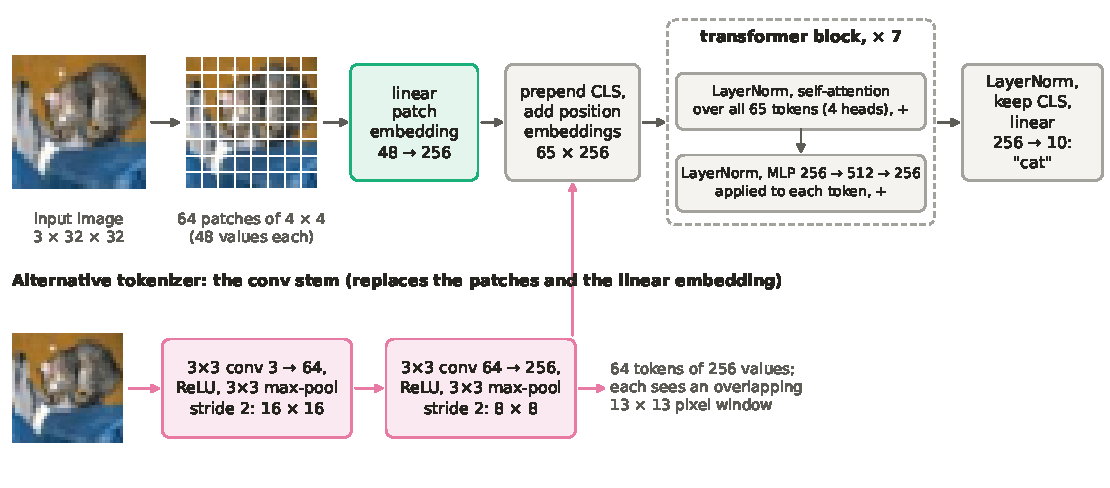
\includegraphics[width=\linewidth]{pipeline.pdf}
\caption{How ViT-Lite-7/4 turns a CIFAR-10 image into a class (top), and the conv stem that replaces the patch embedding in our extension (bottom). The patch-size study changes only the first two boxes of the top row.}
\label{fig:pipeline}
\end{figure}

The Vision Transformer \citep{dosovitskiy2021vit} applies a standard Transformer encoder to an image with almost no image-specific machinery (Figure~\ref{fig:pipeline}). An image of $H\times W$ pixels is cut into $N = HW/P^2$ non-overlapping patches of $P\times P$ pixels. Each patch is flattened into a vector $\mathbf{x}_p^i \in \mathbb{R}^{3P^2}$ and mapped to a $D$-dimensional token by one shared linear map $\mathbf{E}$. A learned class token $\mathbf{x}_{\text{cls}}$ is prepended, and a learned position embedding is added to every token:
\begin{align}
\mathbf{z}_0 &= [\,\mathbf{x}_{\text{cls}};\ \mathbf{x}_p^1\mathbf{E};\ \dots;\ \mathbf{x}_p^N\mathbf{E}\,] + \mathbf{E}_{\text{pos}},
&& \mathbf{E}\in\mathbb{R}^{3P^2\times D},\ \mathbf{E}_{\text{pos}}\in\mathbb{R}^{(N+1)\times D},\\
\mathbf{z}'_\ell &= \mathrm{MSA}(\mathrm{LN}(\mathbf{z}_{\ell-1})) + \mathbf{z}_{\ell-1}, && \ell = 1,\dots,L,\\
\mathbf{z}_\ell &= \mathrm{MLP}(\mathrm{LN}(\mathbf{z}'_\ell)) + \mathbf{z}'_\ell, && \ell = 1,\dots,L,\\
\mathbf{y} &= \mathbf{W}_{\text{head}}\,\mathrm{LN}(\mathbf{z}_L^0).
\end{align}
Each multi-head self-attention (MSA) layer lets every token read from every other token: head $h$ computes $\mathrm{softmax}(\mathbf{Q}_h\mathbf{K}_h^\top/\sqrt{d_h})\,\mathbf{V}_h$ with $d_h = D/\text{heads}$. The MLP acts on each token separately. The prediction $\mathbf{y}$ is read from the class token alone. The cost of attention grows with $N^2$, so halving the patch size multiplies the token count by four and the attention cost by about sixteen.

The contrast with a convolutional network is the point of this project. A convolution looks only at a small neighbourhood and applies the same weights at every position; these two assumptions, locality and weight sharing, are built into the architecture. A ViT has neither in its attention layers. Any token may attend to any other from the first layer onward, and the only hint of spatial layout is the learned position embeddings, which start as random vectors. \citet{dosovitskiy2021vit} found that this weak inductive bias makes ViTs worse than ResNets of similar size when trained on ImageNet-1k, and better only after pretraining on 14 to 300 million images. Figure~\ref{fig:posemb} shows that our small ViT does learn the 2D layout from CIFAR-10 alone: each position's embedding ends up most similar to those of its neighbours, the same pattern \citet{dosovitskiy2021vit} show for their much larger, pretrained ViT.

\begin{figure}[htbp]
\centering
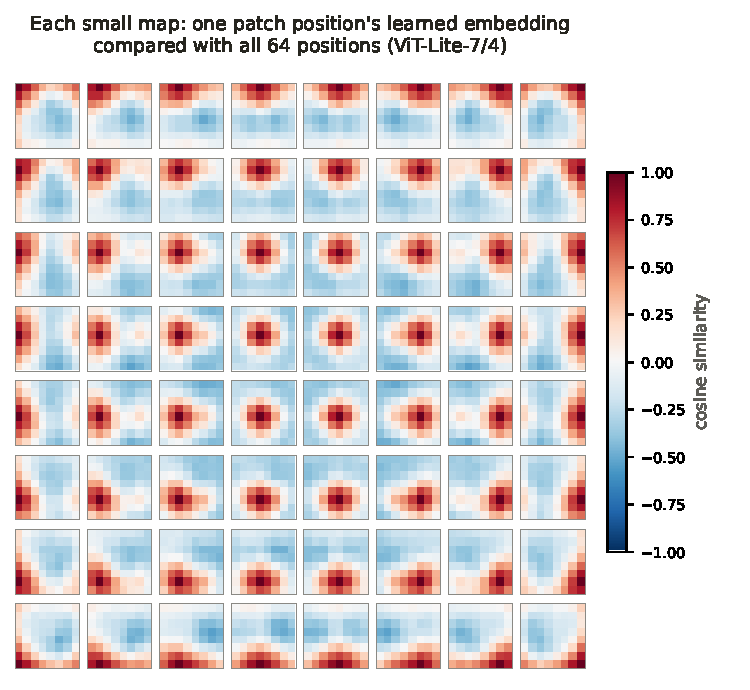
\includegraphics[width=0.55\linewidth]{position_embeddings.pdf}
\caption{Learned position embeddings of ViT-Lite-7/4 (seed 0). Each small map compares one patch position's embedding with all 64 positions (cosine similarity). Nothing tells the model that the patches form an 8$\times$8 grid, yet each embedding is most similar to its neighbours'. Computed from \file{demo/weights/vitlite_p4.safetensors} by \file{experiments/make_figures.py}.}
\label{fig:posemb}
\end{figure}

\subsection{ViT-Lite-7 and the models studied}

ViT-Lite \citep{hassani2021cct} scales the ViT down for small images while keeping its design: $L = 7$ blocks, 4 attention heads, token width $D = 256$ and MLP width 512. With 4$\times$4 patches it has 3.72M parameters, against 86M for ViT-B/16. We build it with the Hugging Face \texttt{ViTForImageClassification} class and a small configuration (\file{src/models.py}), without dropout. Our parameter count matches the 3.72M that \citet{hassani2021cct} report for ViT-Lite-7/4. Table~\ref{tab:models} lists every model in the study. The demo notebook recomputes each step of Figure~\ref{fig:pipeline} by hand from the trained weights and matches the library model to within $4\times10^{-6}$.

\begin{table}[htbp]
\centering
\small
\caption{Models in the study. Tokens include the class token. Forward FLOPs per image are counted with PyTorch's FLOP counter on the actual model definitions (\file{results/model_cost.json}).}
\label{tab:models}
\begin{tabular}{@{}llrrr@{}}
\toprule
Model & Tokenizer & Tokens & Params (M) & GFLOPs/image \\
\midrule
ResNet-18 (baseline) & 3$\times$3 conv stem, stride 1 & n/a & 11.17 & 1.111 \\
ViT-Lite-7/8 & 8$\times$8 patches & 17 & 3.75 & 0.128 \\
ViT-Lite-7/4 & 4$\times$4 patches & 65 & 3.72 & 0.509 \\
ViT-Lite-7/2 & 2$\times$2 patches & 257 & 3.76 & 2.361 \\
ViT-Lite-7 + conv stem & two conv stages & 65 & 3.86 & 0.586 \\
ViT-B/16, pretrained & 16$\times$16 patches at 224 px & 197 & 85.81 & 35.126 \\
\bottomrule
\end{tabular}
\end{table}

The \emph{conv stem} replaces the patches and the linear embedding with two stages of (3$\times$3 convolution, ReLU, 3$\times$3 max-pool with stride 2), going from 3 to 64 to 256 channels. It produces the same 8$\times$8 grid of 64 tokens as 4$\times$4 patches, so the token count and the rest of the network are unchanged. The difference is what a token sees: a 4$\times$4 patch covers 16 pixels with no overlap, while a conv-stem token summarises a 13$\times$13 window that overlaps its neighbours' windows. The \emph{pretrained reference} is \file{google/vit-base-patch16-224-in21k}, pretrained on ImageNet-21k and fine-tuned here on CIFAR-10 with the images resized to 224$\times$224 pixels. It shows what large-scale pretraining buys and serves as a second replication anchor.

\subsection{Related work}

\paragraph{Data and recipes.} The original ViT needs large pretraining datasets to beat CNNs \citep{dosovitskiy2021vit}. DeiT \citep{touvron2021deit} trains ViTs on ImageNet-1k alone by combining strong augmentation, regularization and distillation from a CNN teacher. \citet{steiner2022augreg} show that the right augmentation and regularization can be worth about a tenfold increase in data. Our recipe uses the augmentations of this line of work (RandAugment \citep{cubuk2020randaugment}, Mixup \citep{zhang2018mixup}, CutMix \citep{yun2019cutmix}), but no pretraining or distillation.

\paragraph{Compact transformers for small datasets.} \citet{hassani2021cct} introduce ViT-Lite and two modifications. CVT replaces the class token with \emph{SeqPool}, an attention-weighted average of the output tokens. CCT also replaces the patch embedding with a small convolutional tokenizer. On CIFAR-10 at 300 epochs they report 89.10\% for ViT-Lite-7/8, 93.57\% for ViT-Lite-7/4, 94.01\% for CVT-7/4, 95.04\% for CCT-7/3$\times$2 and 96.53\% for CCT-7/3$\times$1. Their work is the source of our model, our training recipe and our replication anchor.

\paragraph{Putting locality back.} Several papers restore the locality a ViT lacks. \citet{xiao2021early} replace the patch embedding with a few convolutions and find that ViTs then train more stably and reach higher accuracy, which is the idea behind our conv-stem extension. ConViT \citep{dascoli2021convit} initializes attention heads to behave like convolutions and lets each head learn how far to depart from that. \citet{lee2021spt} target small datasets directly with shifted patch tokenization and locality self-attention.

\paragraph{Patch size as a compute lever.} FlexiViT \citep{beyer2023flexivit} trains one model across patch sizes and confirms that smaller patches buy accuracy with compute. \citet{nguyen2024pixels} take this to the limit of one token per pixel. Our study measures the same trade-off at 32 pixels, from scratch, against a tuned CNN.

\paragraph{Analysis tools.} \citet{dosovitskiy2021vit} measure the \emph{mean attention distance} of each head, the average image distance between a token and the tokens it attends to, weighted by attention. \citet{raghu2021see} use it, together with representation similarity, to compare ViTs with CNNs and to study the effect of pretraining dataset scale on intermediate features. We reuse attention distance in Section~\ref{sec:analysis}, alongside layer knockout and linear probes.

\subsection{Claim and research questions}

Our approved claim (approved on November 12, 2026) is:

\begin{quote}
\emph{We claim that a small Vision Transformer trained from scratch on CIFAR-10 stays at least 1 accuracy point below a ResNet-18 at every patch size we test (8x8, 4x4 and 2x2 pixels), and we will test it against a ResNet-18 baseline trained with the same data, augmentation and 300-epoch budget on CIFAR-10.}
\end{quote}

\noindent Around the claim we ask four questions. \textbf{RQ1:} does any patch size bring the ViT within 1 point of ResNet-18? \textbf{RQ2:} what does each patch size cost, and what do the small patches buy at equal compute? \textbf{RQ3:} layer by layer, what does the from-scratch ViT fail to learn? \textbf{RQ4:} does a convolutional stem do better than smaller patches?

%=============================================================================================
\section{Baseline}\label{sec:baseline}

\paragraph{Choice.} The baseline is ResNet-18 \citep{he2016resnet} in its usual CIFAR form: a 3$\times$3 convolution stem with stride 1 and no max-pool, then 8 residual blocks in 4 stages of 64, 128, 256 and 512 channels, global average pooling and a linear head (11.17M parameters). It is the first network most practitioners would train on CIFAR-10, and its convolutions build in exactly the locality and weight sharing that the ViT lacks, which is the contrast the claim is about.

\paragraph{A fair chance.} Both model families are trained with the same data, augmentation, batch size and number of epochs (Table~\ref{tab:recipe}). Each uses its customary optimizer, AdamW for the ViTs and SGD with Nesterov momentum for ResNet-18, and each gets its learning rate tuned with the same two-stage protocol on a 5,000-image validation split carved out of the training set (Table~\ref{tab:lr}). The test set was used only for the final runs. In the first stage, a 30-epoch sweep favoured the smallest rate in the grid for both models. This is the known short-horizon bias of short runs toward small step sizes \citep{wu2018shorthorizon}, so a second stage repeated the check at the full 300 epochs, which decided: 0.025 for ResNet-18 and $2.75\times10^{-4}$ for the ViTs (\file{experiments/decisions.md}). The same rate is used for every ViT variant; it was tuned on ViT-Lite-7/4.

\begin{table}[htbp]
\centering
\small
\caption{Training recipe (\file{experiments/configs/}). Everything above the middle rule is shared by all from-scratch models.}
\label{tab:recipe}
\begin{tabular}{@{}>{\raggedright\arraybackslash}p{2.5cm}>{\raggedright\arraybackslash}p{6.3cm}>{\raggedright\arraybackslash}p{6.3cm}@{}}
\toprule
 & ViT-Lite-7 (all variants) & ResNet-18 \\
\midrule
Data & \multicolumn{2}{>{\raggedright\arraybackslash}p{13.0cm}}{CIFAR-10 \citep{krizhevsky2009cifar}: 50,000 training and 10,000 test images, 32$\times$32 pixels} \\
Augmentation & \multicolumn{2}{>{\raggedright\arraybackslash}p{13.0cm}}{Random resized crop (scale 0.8 to 1), horizontal flip, RandAugment (2 operations, magnitude 9); Mixup ($\alpha=0.8$) or CutMix ($\alpha=1.0$) chosen at random per batch until epoch 175; label smoothing 0.1} \\
Budget & \multicolumn{2}{>{\raggedright\arraybackslash}p{13.0cm}}{300 epochs, batch size 128, bfloat16 autocast, one A100 MIG 2g.10gb slice on Wulver; 3 seeds} \\
\midrule
Optimizer & AdamW, weight decay 0.06 & SGD, Nesterov momentum 0.9, weight decay $5\times10^{-4}$ \\
Learning rate & $2.75\times10^{-4}$ (selected, Table~\ref{tab:lr}) & 0.025 (selected, Table~\ref{tab:lr}) \\
Schedule & 10 warmup epochs, cosine decay to $10^{-5}$, 10 cooldown epochs & 5 warmup epochs, cosine decay to 0 \\
Model regularization & none (no dropout, no stochastic depth) & batch normalization \\
\bottomrule
\end{tabular}
\end{table}

\begin{table}[htbp]
\centering
\small
\caption{Learning-rate selection: validation accuracy (\%) on the 5,000-image validation split, seed 0. The largest value in each row is in bold. The 300-epoch check decided.}
\label{tab:lr}
\begin{tabular}{@{}llccc@{}}
\toprule
Model & Run length & \multicolumn{3}{c}{Learning rate: validation accuracy} \\
\midrule
\multirow{2}{*}{ResNet-18} & 30 epochs & 0.05: \textbf{93.38} & 0.1: 92.86 & 0.2: 92.62 \\
 & 300 epochs & 0.025: \textbf{96.08} & 0.05: 95.82 & 0.1: 95.80 \\
\multirow{2}{*}{ViT-Lite-7/4} & 30 epochs & $2.75\times10^{-4}$: \textbf{75.56} & $5.5\times10^{-4}$: 67.84 & $1.1\times10^{-3}$: 64.18 \\
 & 300 epochs & $1.375\times10^{-4}$: 90.48 & $2.75\times10^{-4}$: \textbf{91.22} & $5.5\times10^{-4}$: 90.20 \\
\bottomrule
\end{tabular}
\end{table}

\paragraph{Result.} ResNet-18 reaches $96.10 \pm 0.13\%$ test accuracy over three seeds (96.25, 95.99 and 96.07\%) in 1.09 GPU-hours per run (\file{results/summary.md}). All accuracies in this report are taken at the final epoch; taking the best evaluated epoch instead would add only 0.03~points for ResNet-18. Its learning curve leads every ViT throughout training: after 10 epochs it is at 81.74\%, against 58.61\% for ViT-Lite-7/4, and after 100 epochs at 91.94\% against 87.00\% (Figure~\ref{fig:curves}, \file{results/figures/figures.md}). The comparison is not one-sided in the ResNet's favour on every axis, and we state both directions: ResNet-18 has three times the parameters of ViT-Lite-7, while ViT-Lite-7/2 uses 2.1 times ResNet-18's FLOPs per image and is still 4.39~points behind.

%=============================================================================================
\section{Replication Anchor}\label{sec:anchor}

We compare our models with three published numbers (Table~\ref{tab:anchor}). The pretrained ViT-B/16 is a faithful replication. \citet{dosovitskiy2021vit} report 98.95\% for ViT-B/16 pretrained on ImageNet-21k and fine-tuned at 384 pixels; we fine-tune at 224 pixels for only 5 epochs and reach 98.77\%, 0.18~points lower, in 0.44 GPU-hours. The demo notebook reloads the fine-tuned weights on Wulver and reproduces exactly this number.

\begin{table}[htbp]
\centering
\small
\caption{Replication anchors. Final-epoch test accuracy, mean $\pm$ standard deviation over 3 seeds unless noted (\file{results/summary.md}).}
\label{tab:anchor}
\begin{tabular}{@{}lccc@{}}
\toprule
Model & Ours (\%) & Published (\%) & Difference (points) \\
\midrule
ViT-Lite-7/8 & $87.96 \pm 0.29$ & 89.10 \citep{hassani2021cct} & $-1.14$ \\
ViT-Lite-7/4 & $91.57 \pm 0.49$ & 93.57 \citep{hassani2021cct} & $-2.00$ \\
ViT-B/16, pretrained, fine-tuned (1 seed) & 98.77 & 98.95 \citep{dosovitskiy2021vit}, at 384 px & $-0.18$ \\
\bottomrule
\end{tabular}
\end{table}

ViT-Lite, trained with what we took to be the released recipe, lands 1.14 and 2.00~points below the published values. We investigated the gap in the following order.

\begin{enumerate}[leftmargin=*]
\item \textbf{Reporting convention.} We report the final epoch. Reporting the best evaluated epoch would raise our numbers by only 0.12 (7/8) and 0.35~points (7/4), so the convention explains little of the gap.
\item \textbf{Learning rate.} We use $2.75\times10^{-4}$ instead of the published $5.5\times10^{-4}$. At 300 epochs on the validation split, $5.5\times10^{-4}$ scored 1.02~points lower (Table~\ref{tab:lr}, one seed), so our choice should not cost accuracy.
\item \textbf{Seed noise.} Even our best ViT-Lite-7/4 seed (91.97\%) is 1.60~points below 93.57\%, so the gap is not seed-to-seed variation.
\item \textbf{Regularization inside the model.} When we re-read the released code \citep{cctrepo}, we found that its ViT-Lite uses attention dropout 0.1 and stochastic depth 0.1 by default, set in the model definition rather than in the training config. Our Hugging Face model uses neither. Given how much regularization matters for ViTs on small data \citep{steiner2022augreg}, we consider this the most likely cause of the gap. We have not tested it.
\item \textbf{Augmentation implementation.} The released config uses the \texttt{timm} RandAugment policy \texttt{rand-m9-}\allowbreak\texttt{mstd0.5-inc1} with random interpolation; we use torchvision's RandAugment with 2 operations at magnitude 9. The idea is the same but the operations and their strengths differ.
\end{enumerate}

\noindent The conv-stem model gives a third, indirect check. CCT-7/3$\times$2, which tokenizes with two convolutional layers at the same cost as our conv stem (0.29 GMACs per image for both; our 0.586 GFLOPs count each multiply-add as two operations), reports 95.04\%. Our conv stem reaches $93.08 \pm 0.22\%$, 1.96~points lower. It is not an exact replication, since CCT uses SeqPool where we use a class token, but the gap matches the 2.00~points of ViT-Lite-7/4. This points to a difference shared by all our ViTs, such as items 4 and 5, rather than a bug in one model. Because all our ViT variants share the recipe, this offset does not affect the comparisons between them, and Section~\ref{sec:verdict} shows that it does not change the verdict on the claim.

%=============================================================================================
\section{Perturbation Study}\label{sec:perturbation}

\paragraph{Setup.} The controlled change is the tokenizer, varied as a sensitivity sweep over the patch size: 8$\times$8, 4$\times$4 and 2$\times$2 pixels (16, 64 and 256 tokens). Everything else is held fixed: the 7 transformer blocks, the data and augmentation, the optimizer, the learning rate and the 300 epochs. Each setting is trained with 3 seeds, and accuracy is measured once, at the final epoch, on the test set. All runs were Wulver batch jobs; the job scripts and logs are in \file{experiments/wulver/}. Two extensions complete the picture: the conv stem of Section~\ref{sec:model} (RQ4), and a compute-matched run that gives the 2$\times$2 model the training FLOPs of the 4$\times$4 model (RQ2). The 2$\times$2 model costs 4.64 times the forward FLOPs per image (Table~\ref{tab:models}), so it was trained for $300/4.64 \approx 65$ epochs, with the warmup, cooldown and Mixup switch-off epoch scaled in proportion. Both extensions were set up before their results were seen (\file{experiments/decisions.md}).

\begin{table}[htbp]
\centering
\small
\caption{Main results. Final-epoch test accuracy over 3 seeds; training compute is forward GFLOPs per image $\times$ 50,000 images $\times$ epochs (\file{results/figures/figures.md}). GPU-hours are measured per run on one A100 MIG 2g.10gb slice.}
\label{tab:main}
\begin{tabular}{@{}lcccrr@{}}
\toprule
Model & Test accuracy (\%) & Per seed (\%) & Gap to ResNet-18 & PFLOP & GPU-h \\
\midrule
ResNet-18 & $96.10 \pm 0.13$ & 96.25, 95.99, 96.07 & n/a & 16.7 & 1.09 \\
\midrule
ViT-Lite-7/8 & $87.96 \pm 0.29$ & 88.14, 87.62, 88.11 & 8.15 & 1.9 & 0.95 \\
ViT-Lite-7/4 & $91.57 \pm 0.49$ & 91.71, 91.97, 91.02 & 4.54 & 7.6 & 1.04 \\
ViT-Lite-7/2 & $91.71 \pm 0.35$ & 91.50, 91.52, 92.11 & 4.39 & 35.4 & 3.42 \\
\midrule
ViT-Lite-7 + conv stem & $93.08 \pm 0.22$ & 92.93, 92.99, 93.33 & 3.02 & 8.8 & 1.00 \\
ViT-Lite-7/2, 65 epochs & $78.53 \pm 1.02$ & 78.30, 79.65, 77.65 & 17.57 & 7.7 & 0.67 \\
\bottomrule
\end{tabular}
\end{table}

\begin{figure}[htbp]
\centering
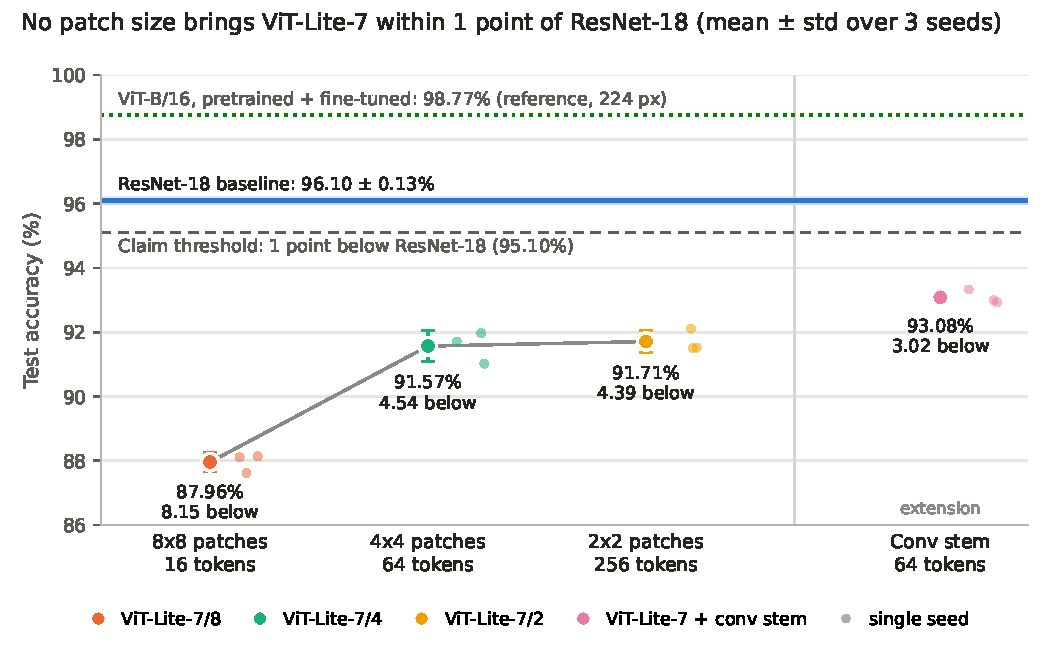
\includegraphics[width=0.9\linewidth]{claim.pdf}
\caption{Test accuracy against patch size (mean $\pm$ standard deviation over 3 seeds; small dots are single seeds). The blue line and band are ResNet-18; the dashed line is the claim's threshold, 1 point below it. No patch size reaches the threshold, and neither does the conv stem.}
\label{fig:claim}
\end{figure}

\paragraph{Patch size.} Table~\ref{tab:main} and Figure~\ref{fig:claim} give the results. Going from 8$\times$8 to 4$\times$4 patches adds 3.61~points. Going from 4$\times$4 to 2$\times$2 adds 0.14~points, which is within the seed standard deviation of either model (0.35 to 0.49), for 4.64 times the FLOPs and 3.3 times the GPU time. Finer patches stop paying off at 4$\times$4: the 2$\times$2 model sees each pixel group in more detail but gets no better at the task.

\paragraph{Equal compute.} With the same training FLOPs as the 4$\times$4 model, the 2$\times$2 model reaches $78.53 \pm 1.02\%$, 13.04~points below it (Figure~\ref{fig:compute}). Two caveats, recorded before the analysis in \file{experiments/decisions.md}, limit this comparison. First, the 65-epoch run reuses the learning rate chosen at 300 epochs, and the 30-epoch sweep showed how much short schedules hurt ViT-Lite (75.56\% validation accuracy after 30 epochs against 91.22\% after 300), so part of the 13-point drop is a short-schedule penalty rather than an effect of patch size alone. Second, the match is in FLOPs, not in time: on our GPU slice the run took 0.67 hours against 1.04 for the 4$\times$4 model, because the larger matrices of the 2$\times$2 model use the hardware more efficiently. Plotted against cumulative training compute (Figure~\ref{fig:curves}, right), the 2$\times$2 model trails the 4$\times$4 model at every point of training.

\begin{figure}[htbp]
\centering
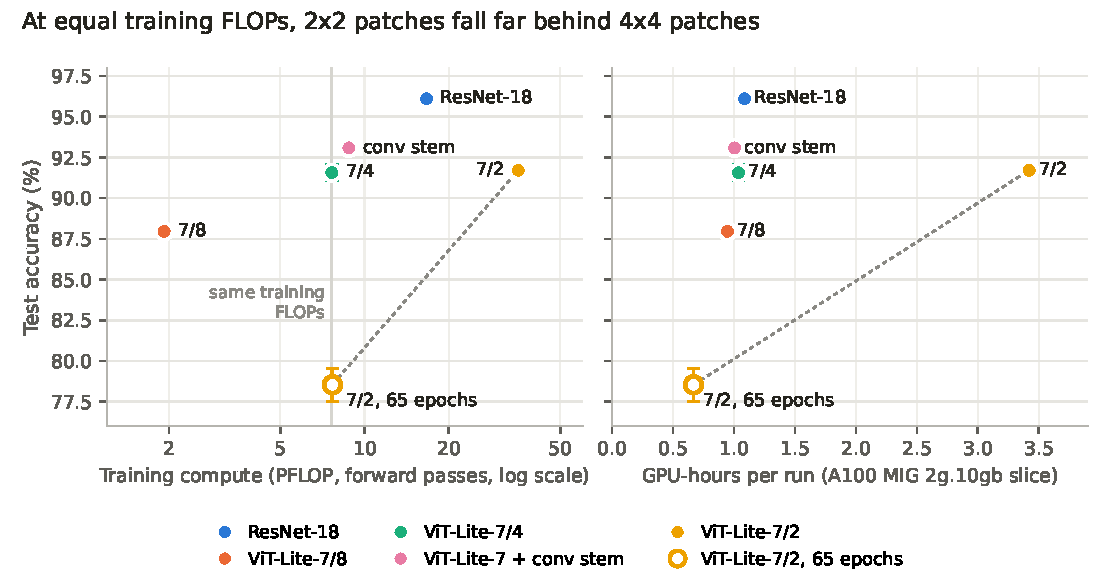
\includegraphics[width=\linewidth]{compute.pdf}
\caption{Test accuracy against training compute (left, log scale) and against measured GPU-hours per run (right). The hollow marker is the 2$\times$2 model trained for 65 epochs, which has the same training FLOPs as the 4$\times$4 model; the dotted line joins it to the 300-epoch 2$\times$2 model.}
\label{fig:compute}
\end{figure}

\begin{figure}[htbp]
\centering
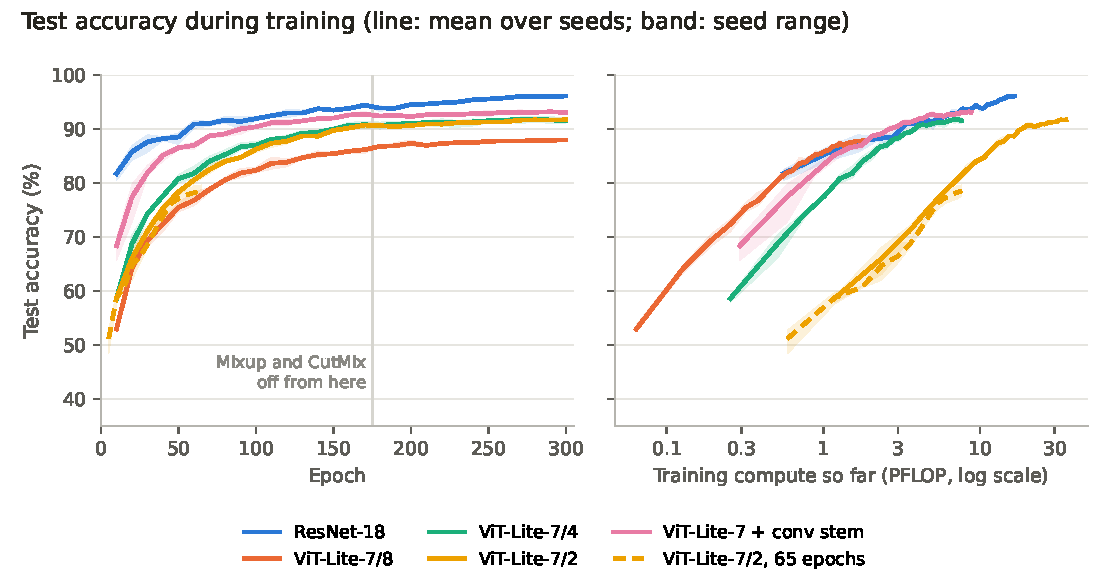
\includegraphics[width=\linewidth]{curves.pdf}
\caption{Test accuracy during training, evaluated every 10 epochs (every 5 for the 65-epoch run); line: mean over seeds, band: seed range. Left: by epoch, with Mixup and CutMix switched off at epoch 175. Right: by cumulative training compute.}
\label{fig:curves}
\end{figure}

\paragraph{The conv stem.} Replacing the patches with the conv stem gives $93.08 \pm 0.22\%$, the best result of any ViT we trained from scratch. It beats 4$\times$4 patches, which have the same 64 tokens, by 1.51~points for 15\% more FLOPs, and beats 2$\times$2 patches by 1.37~points with a quarter of their FLOPs and under a third of their GPU time. This agrees with \citet{xiao2021early}. It still falls 3.02~points short of ResNet-18.

%=============================================================================================
\section{Analysis and Outlook}\label{sec:analysis}

\subsection{Verdict: the claim holds}\label{sec:verdict}

ResNet-18 leads ViT-Lite-7 by 8.15, 4.54 and 4.39~points at patch sizes 8, 4 and 2 (Table~\ref{tab:main}). Each gap is far above the 1-point margin of the claim and at least 9 times the largest seed standard deviation (0.49). The verdict survives the most pessimistic pairing of seeds: the lowest ResNet-18 seed (95.99\%) minus the best ViT seed still leaves 7.85, 4.02 and 3.88~points. It also survives the replication gap of Section~\ref{sec:anchor}: even if the ViTs gained the full 2.00~points by which ViT-Lite-7/4 trails its published value, the gaps at 4$\times$4 and 2$\times$2 would be 2.54 and 2.39~points. Beyond the claim, the conv stem stays 3.02~points behind (2.66 in the worst seed pairing). \textbf{The claim holds at every patch size tested}, and we answer RQ1 with no: on CIFAR-10 at this scale, a from-scratch ViT does not reach ResNet-18 by changing its patch size.

\subsection{Where the model breaks}

\paragraph{By class.} The ViTs lose most on animals (Figure~\ref{fig:perclass}). Against ResNet-18, ViT-Lite-7/4 is 9.97~points lower on cat, 7.97 on dog, 6.30 on bird and 5.83 on deer, but only 1.60 on truck and 1.63 on frog. Cat confused with dog is the most frequent error for every model, ResNet-18 included. A ViT-specific error is cat predicted as frog: it is among the four most frequent confusions of the ViTs (99 test images for ViT-Lite-7/4 over three seeds) but not of ResNet-18 (\file{results/figures/figures.md}). The classes that suffer are those told apart by fine local shape and texture rather than by colour and global layout, which is what the layer analyses below point to.

\begin{figure}[htbp]
\centering
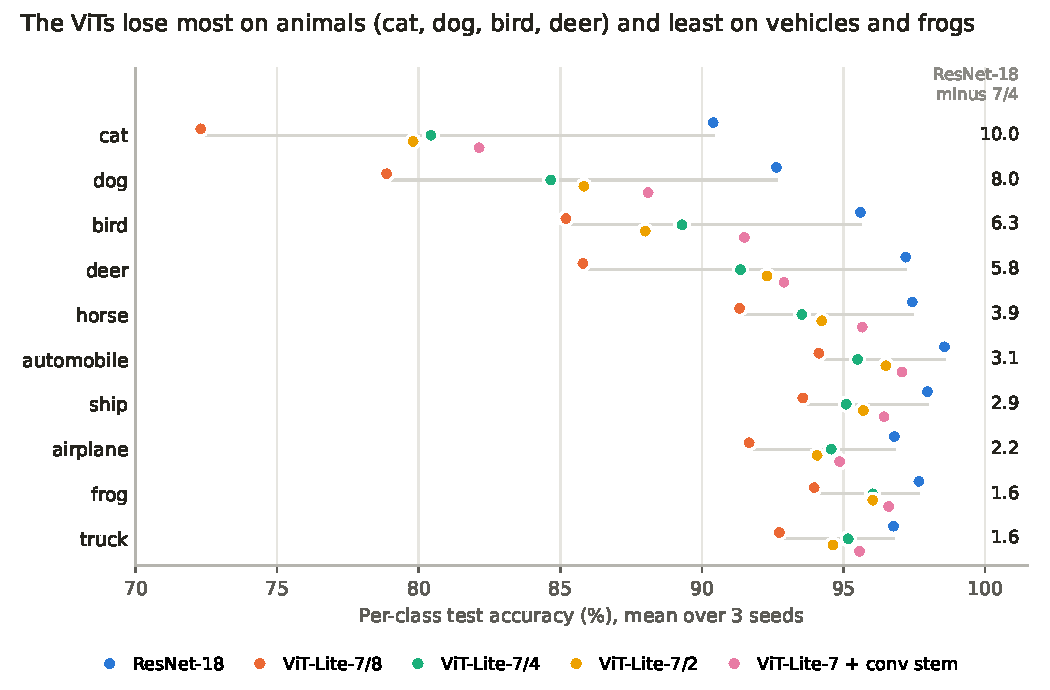
\includegraphics[width=0.88\linewidth]{per_class.pdf}
\caption{Per-class test accuracy (mean over 3 seeds), classes sorted by the gap between ResNet-18 and ViT-Lite-7/4 (right column).}
\label{fig:perclass}
\end{figure}

\paragraph{By layer: attention distance.} Figure~\ref{fig:attention} shows the mean attention distance of each layer, measured between patch tokens over 1,000 test images (\file{results/analysis/attention_distance.md}). In the first layer, the from-scratch ViTs attend almost uniformly: 14.7, 15.0 and 15.1 pixels for patch sizes 8, 4 and 2, close to the 16.1 to 16.7 pixels that uniform attention would give. Locality appears only in layer 2, the most local layer of every from-scratch ViT (11.9, 10.7 and 8.5 pixels; the most local head reaches 8.2, 6.1 and 4.2). The pretrained ViT-B/16 is different: already in layer 1 it has heads at 0.0 pixels, attending to their own patch, and its layers 2 and 3 average 8.4 and 9.3 pixels. Fine-tuning on CIFAR-10 changes these distances little (layer 1: 10.9 pixels before fine-tuning, 11.2 after), so the locality comes from pretraining.

\begin{figure}[htbp]
\centering
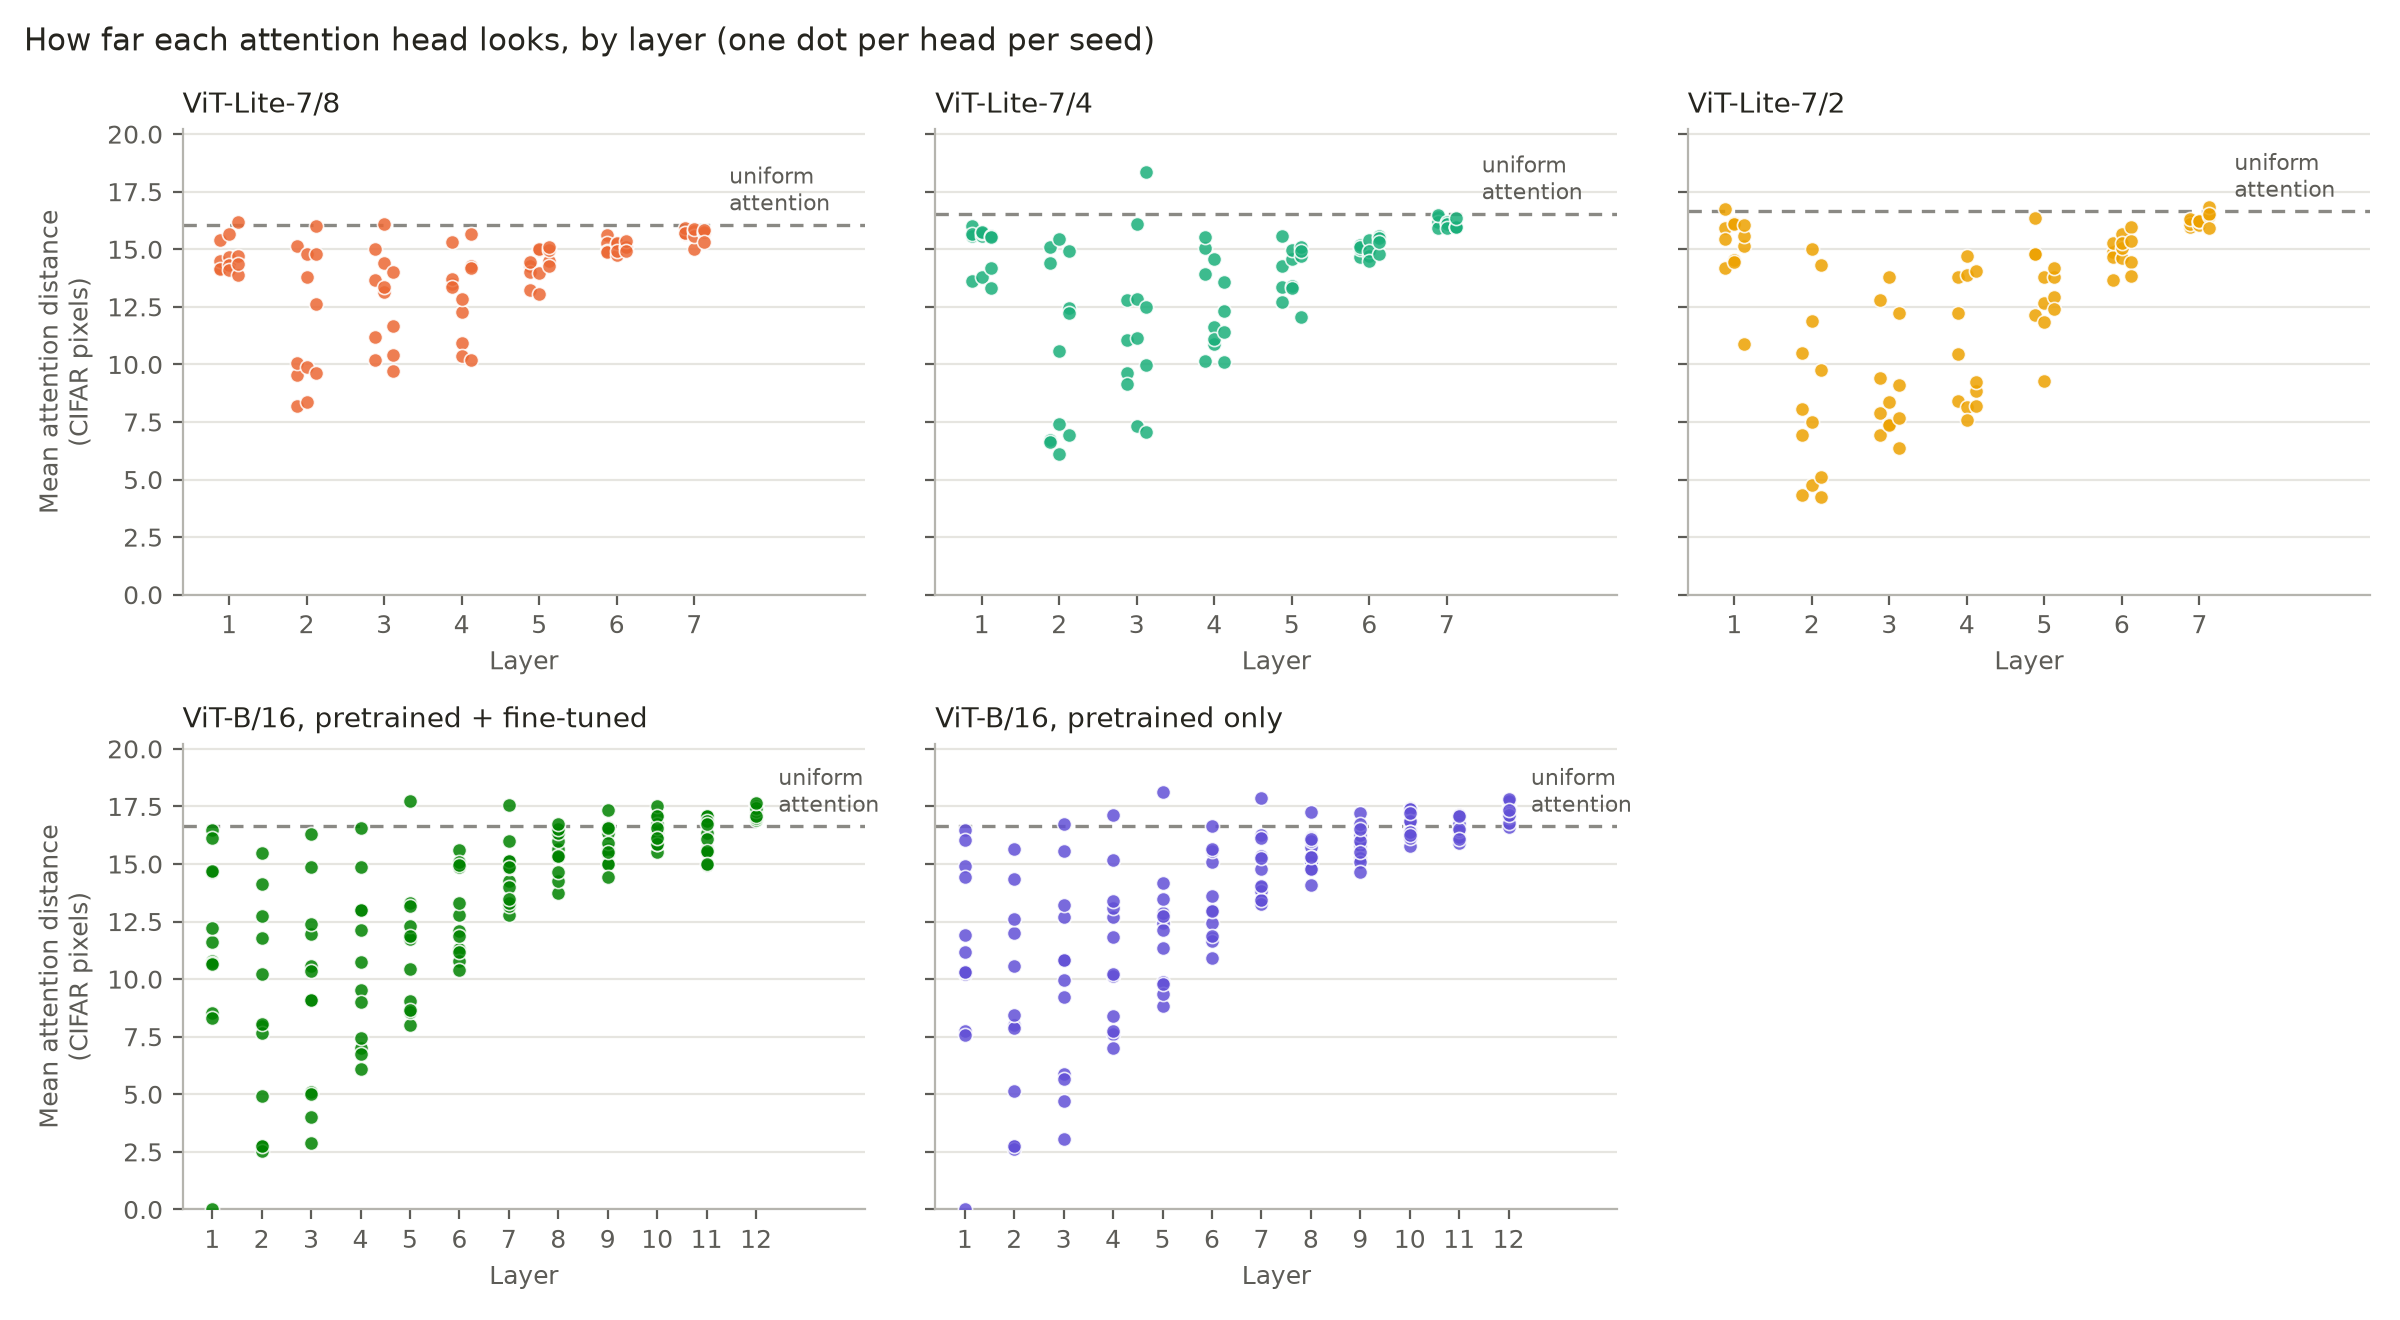
\includegraphics[width=\linewidth]{attention_distance.png}
\caption{Mean attention distance of every head, by layer, in CIFAR pixels, over the first 1,000 test images; one dot per head and seed. The dashed line is the distance under uniform attention. Produced by \file{src/analysis/attention_distance.py}.}
\label{fig:attention}
\end{figure}

\paragraph{By layer: knockout.} Figure~\ref{fig:knockout} removes one sub-layer at a time at test time and measures the accuracy drop (\file{results/analysis/knockout.md}). The from-scratch ViTs depend heavily on their first two blocks. Removing the block-1 MLP costs 77.67, 80.39 and 82.45~points for patch sizes 8, 4 and 2, which is close to chance. Removing the layer-2 attention costs 4.23, 11.26 and 34.04~points, more the smaller the patch: with 2$\times$2 patches, each token holds only 12 numbers, and layer-2 attention is where neighbouring tokens are combined into usable local features. Blocks 3 to 7 cost 3.82 to 7.84~points each for 4$\times$4 patches and 7.41 to 11.69 for 2$\times$2. The pretrained ViT-B/16 spreads its work more evenly: apart from block 1 (86.56) and block 2 (8.53), no block costs more than 2.61~points.

\begin{figure}[htbp]
\centering
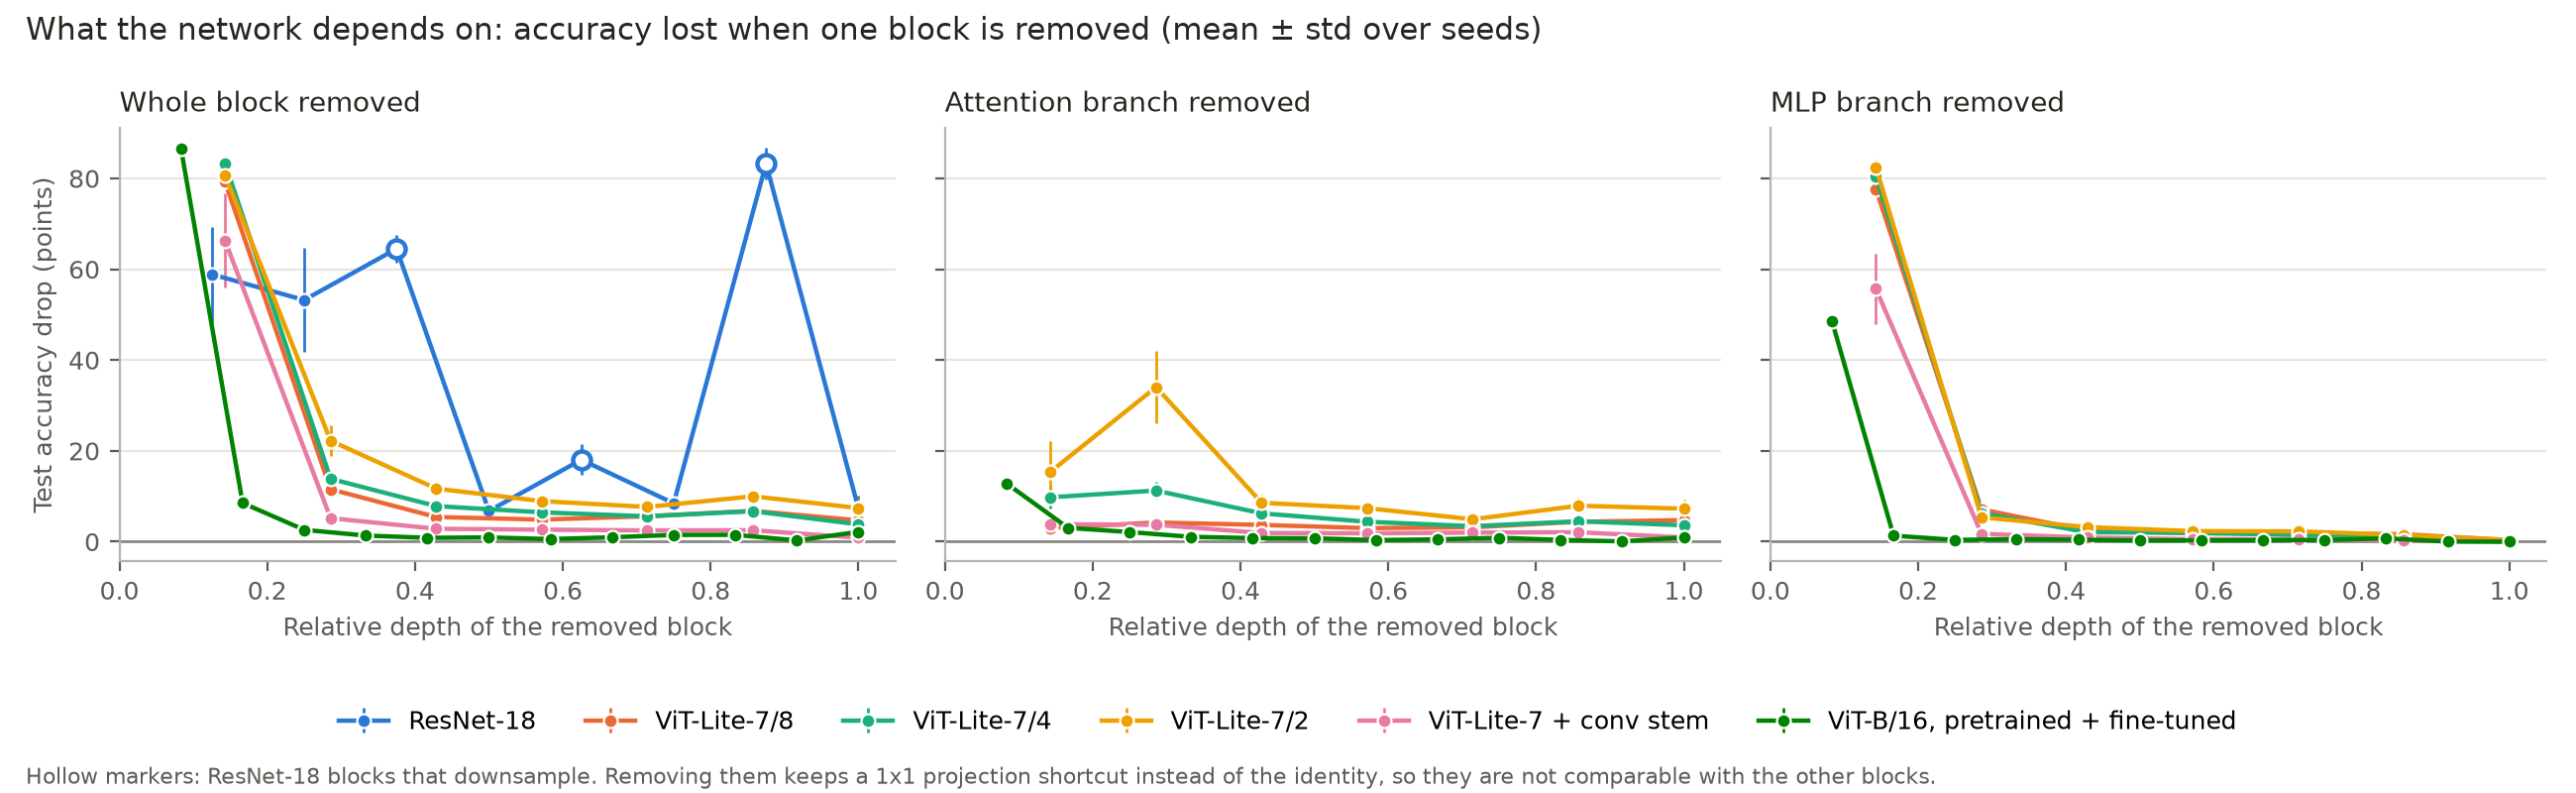
\includegraphics[width=\linewidth]{knockout.png}
\caption{Accuracy drop when one block (left), one attention branch (middle) or one MLP branch (right) is removed at test time, mean over seeds. For ResNet-18, hollow markers are downsampling blocks, whose removal leaves a projection shortcut and is not comparable. Produced by \file{src/analysis/knockout.py}.}
\label{fig:knockout}
\end{figure}

\paragraph{By layer: linear probes.} Figure~\ref{fig:probes} fits a logistic regression on frozen features after each layer (\file{results/analysis/probes.md}). Before any transformer block, the average of the patch tokens predicts the class with 29.60\% accuracy for 4$\times$4 patches, against 49.53\% after ResNet-18's single stem convolution: a linear map of raw pixels carries little class information. After block 1, the class token of ViT-Lite-7/4 reaches 46.75\%, against 53.53\% for the pretrained ViT-B/16. The ViTs then gain steadily, and their final class-token probes (87.84, 91.63 and 91.69\%) match their test accuracy.

\begin{figure}[htbp]
\centering
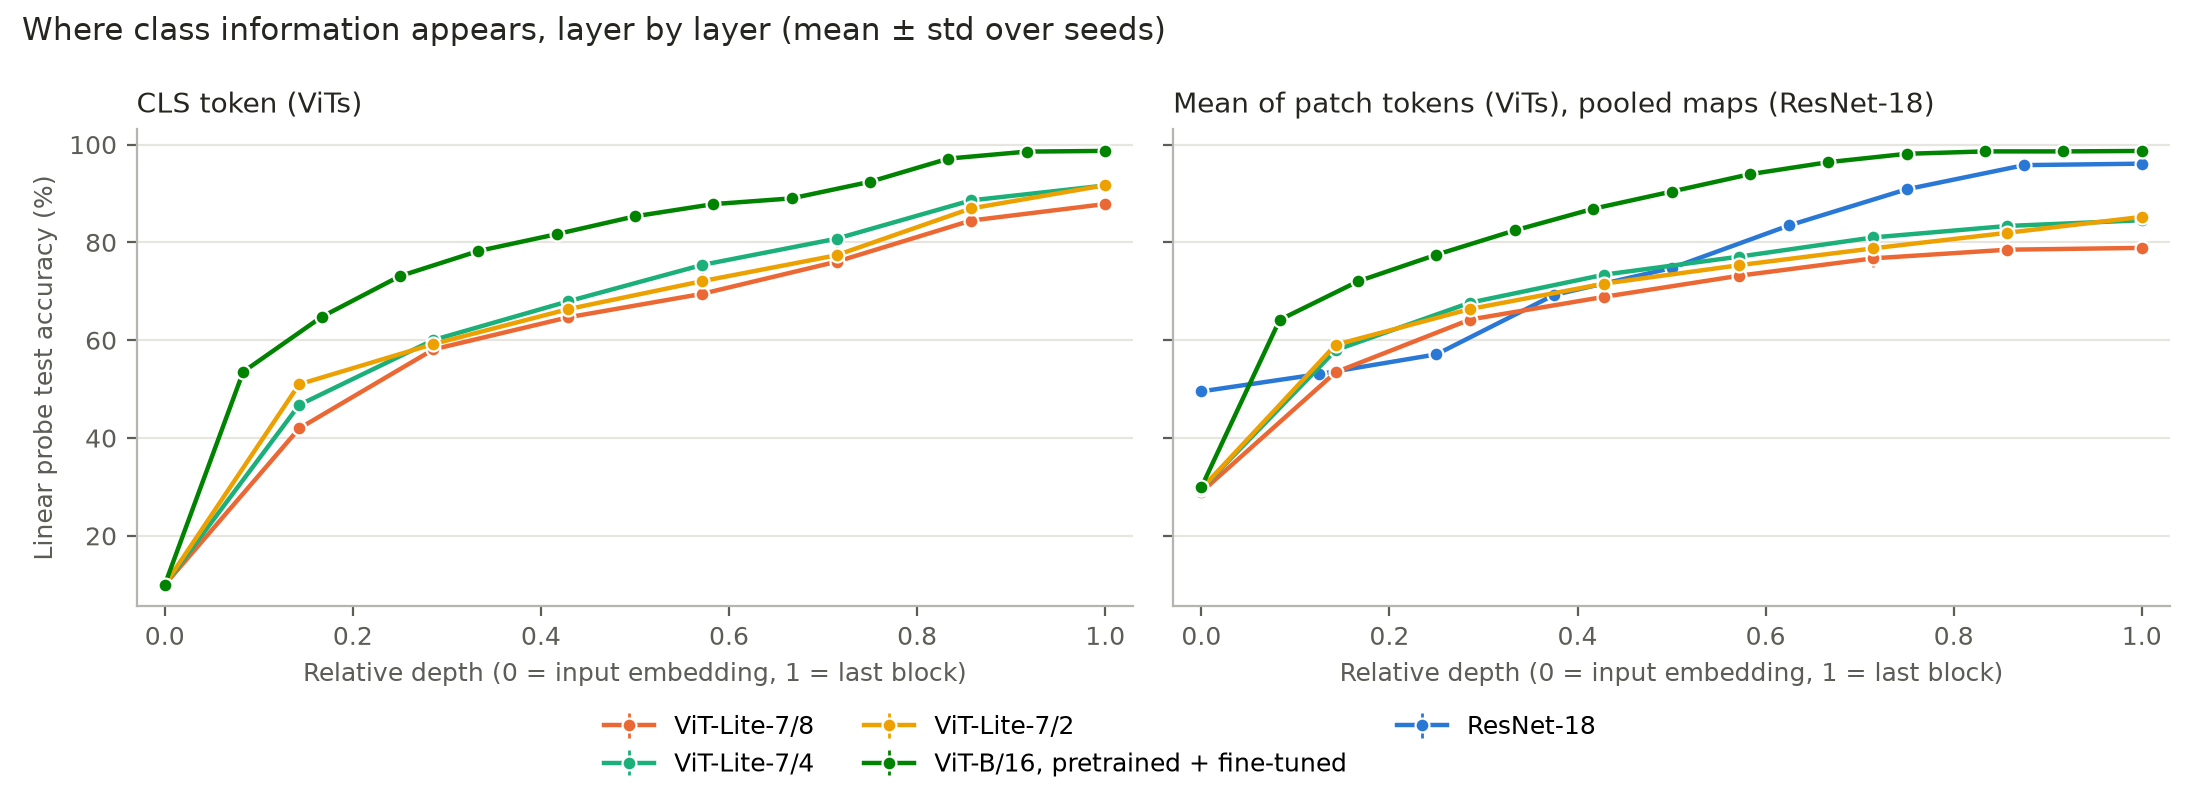
\includegraphics[width=\linewidth]{probes.png}
\caption{Linear-probe test accuracy by relative depth, for the class token (left) and the mean of the patch tokens or ResNet-18's pooled feature map (right), mean over seeds. Produced by \file{src/analysis/probes.py}.}
\label{fig:probes}
\end{figure}

\paragraph{What the conv stem changes.} One might expect the conv stem to help by making attention local. It does the opposite. Its attention is \emph{less} local than with patches (layer 2: 12.3 pixels, against 10.7 for 4$\times$4 patches), because the stem already does the local work: its tokens probe at 65.06\% before any transformer block, more than ResNet-18's stem (49.53\%). With that work done, the network depends far less on any single part. Removing the block-1 MLP costs 55.68~points instead of 80.39, close to ViT-B/16's 48.63; no attention branch costs more than 3.85~points; and each block after the first costs 0.89 to 5.18. The conv stem's lead over 4$\times$4 patches is largest early and shrinks with depth: 22.98~points in the class-token probe after block 1 (69.73 against 46.75\%), 1.50~points after block 7 (93.13 against 91.63\%). ResNet-18, meanwhile, keeps improving in its deep layers: its pooled features rise from 83.47\% after block 5 to 96.09\% after block 8, while the conv-stem patch tokens rise from 84.07\% after block 4 to 88.80\% after block 7. We read this as follows. The from-scratch ViT's first handicap is at the input, where it must learn locality from data, and a conv stem removes it. What remains of the gap opens in the deeper layers, where ResNet-18 keeps building features and the small ViT, without pretraining, does not.

\subsection{Limitations}

The study uses one dataset at 32 pixels and three seeds per model, with one seed for ViT-B/16. The ViT learning rate was tuned only on ViT-Lite-7/4 and shared by all variants, which could disadvantage the others slightly. Our ViTs lack the attention dropout and stochastic depth of the reference implementation (Section~\ref{sec:anchor}), so absolute ViT accuracies are likely 1 to 2~points low; this does not change the verdict. The compute-matched run has the two caveats of Section~\ref{sec:perturbation}. The layer analyses use the final checkpoint of each seed and the first 1,000 (attention distance) or all 10,000 (knockout, probes) test images.

\subsection{Outlook}

\paragraph{Next experiments.} Three experiments follow directly. First, adding stochastic depth 0.1 and attention dropout 0.1 to ViT-Lite-7/4 and the conv-stem model would test the replication gap and show how much of the remaining 3 points regularization can close (about 3 GPU-hours per model on our hardware). Second, SeqPool \citep{hassani2021cct} or shifted patch tokenization \citep{lee2021spt} would test whether the deeper-layer gap is about how information is pooled. Third, training a single model across patch sizes, as in FlexiViT \citep{beyer2023flexivit}, would give the whole accuracy-against-compute curve from one training run.

\paragraph{Applications.} The result matters most where pretraining data do not exist or do not transfer: small, low-resolution image collections such as microscopy and histopathology tiles, astronomical cutouts, particle-detector images and low-resolution satellite tiles. There, the choice between a CNN, a conv-stem ViT and a pretrained ViT is a real engineering decision, and our results suggest starting from a conv stem rather than smaller patches. Patch size can also serve as a deployment knob on small devices: ViT-Lite-7/8 uses 0.128 GFLOPs per image, about one ninth of ResNet-18's, for a known accuracy cost. Finally, the knockout and probe analyses are cheap diagnostics that could be run on any ViT before deployment. Near-uniform first-layer attention and heavy dependence on block 1 flag a model that is still missing locality, and therefore one that would likely benefit from a convolutional stem or from pretraining.

\paragraph{Reproducibility.} All training ran on one A100 MIG 2g.10gb slice of NJIT's Wulver cluster, about 31 GPU-hours in total for the learning-rate sweeps and the final runs. The repository README lists the commands that reproduce every table and figure in this report, and the demo notebook (\file{demo/demo.ipynb}) walks through each model's computation on real test images and reproduces the test accuracy of each exported model.

\FloatBarrier
\bibliographystyle{plainnat}
\bibliography{references}

\end{document}
